\pr Comme nous l'avons appris du Sauveur et selon son commandement, nous osons dire:

\begin{center}
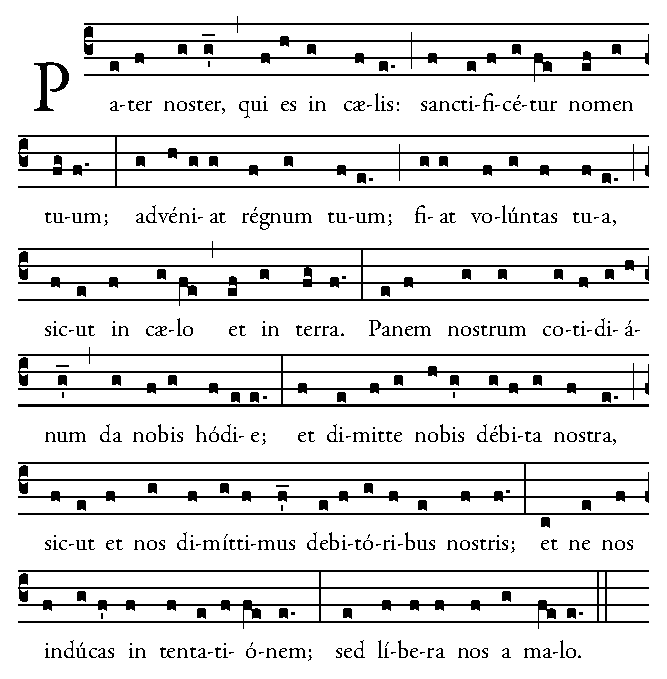
\includegraphics[width=.9\textwidth]{src/ordinario/pater.eps}
\end{center}

\be Notre Père, qui es aux cieux,\redast que ton nom soit sanctifié;\redast que ton règne vienne,\redast que ta volonté soit faite sur la terre comme au ciel.\redast Donne-nous aujourd'hui notre pain de ce jour.\redast Pardonne-nous nos offenses,\redast comme nous pardonnons aussi à ceux qui nous ont offensés.\redast Et ne nous soumets pas à la tentation,\redast mais délivre-nous du Mal.

\pr Délivre-nous de tout mal, Seigneur, et donne la paix à notre temps; par ta miséricorde, libère-nous du péché, rassure-nous devant les épreuves en cette vie où nous espérons le bonheur que tu promets et l’avènement de Jésus Christ, notre Sauveur.

\be Car c'est à toi qu'appartiennent le règne, la puissance et la gloire, pour les siècles des siècles.

\pr Seigneur Jésus Christ, tu as dit à tes Apôtres: «Je vous laisse la paix, je vous donne ma paix»; ne regarde pas nos péchés mais la foi de ton Église; pour que ta volonté s’accomplisse, donne-lui toujours cette paix, et conduis-la vers l'unité parfaite, toi qui règnes pour les siècles des siècles.

\be Amen.

\pr Que la paix du Seigneur soit toujours avec vous.

\be Et avec votre esprit.

\pr Frères, dans la charité du Christ, donnez-vous la paix.

\be Agneau de Dieu, qui enlèves le péché du monde,\redast prends pitié de nous.\\
\indent\be Agneau de Dieu, qui enlèves le péché du monde,\redast prends pitié de nous.\\
\indent\be Agneau de Dieu, qui enlèves le péché du monde,\redast donne-nous la paix.

\pr Heureux les invités au repas du Seigneur! Voici l'Agneau de Dieu qui enlève le péché du monde.

\be Seigneur, je ne suis pas digne de te recevoir; mais dis seulement une parole et je serai guéri.

\pr Prions le Seigneur.

\pr Regarde avec bonté, Seigneur, le peuple que tu as rénové par tes sacrements; Accorde-nous de parvenir à la résurrection bienheureuse, toi qui nous as destinés à connaitre ta gloire. Par Jésus, le Christ, notre Seigneur.

\be Amen.